\subsection{Rappresentazioni di funzioni}

\subsubsection{Funzioni in \texorpdfstring{\(\R^2\)}{R2}}

Consideriamo una funzione \(f: D \subseteq \R^2 \to \R \) che associa \((x,y) \mapsto f(x,y)\).

L'insieme \(D\) è il dominio della funzione, ovvero, l'insieme dei punti \((x,y) \in \R^2\) per cui \(f(x,y) \in \R \)

\[D = \{(x,y) \in \R^2 \giventhat f(x,y) \in \R \} \subseteq \R^2 \]

Definiamo tutti i valori che può assumere la funzione con l'immagine della funzione che è definita come segue:

\[\im{f} = \{z \in \R \giventhat z = f(x,y), ~\forall (x,y) \in D\} \subset \R \]

\subsubsection*{Esempi}

\begin{enumerate}
    \item \(f(x,y) = 3x + 2y + 5 \implies D=\R^2\)
    \item \(f(x,y) = \frac{\ln(x+y)}{x-3}\)
          \begin{align*}
              D & = \{(x,y) \in \R^2 \giventhat x-3 \ne 0;\ x+y > 0\} & \text{(\(x+y > 0 \to \) disequazione in \(\R^2\))} \\
                & = \{(x,y) \in \R^2 \giventhat x \ne 3;\ y > -x\}
          \end{align*}

          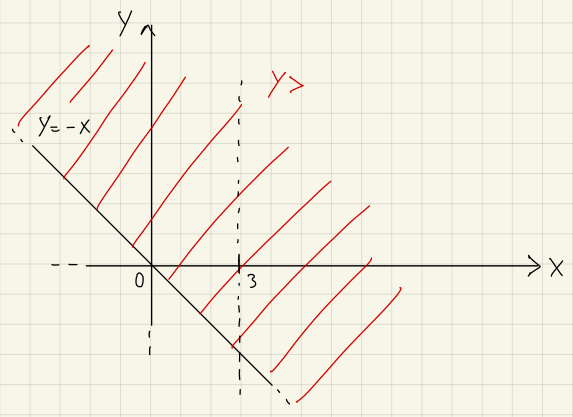
\includegraphics[width=0.5\textwidth]{grafico-di-funzioni-2.png}
\end{enumerate}

\filbreak{}
\subsubsection{Insiemi del piano \texorpdfstring{\(\R^2\)}{R2} determinati da disequazioni}

Consideriamo il caso reale. Sia \(f: I \subset \R \to \R \) continua, definiamo il suo grafico:

\[\graf{f} = \{(x,y) \in \R^2 \giventhat y=f(x),\ x \in I \} = \underbrace{\{(x,f(x))\}}_{\text{con \(x \in I\)}}\]

Possiamo quindi definire il concetto di sopragrafico e sottografico di una funzione:

\defn{Sopragrafico}{
    Si definisce sopragrafico la parte di piano tale che:

    \[y \ge f(x) \implies \{(x,y) \in \R^2 \giventhat x \in I;\ y \ge f(x) \} \]

    Oppure, nella forma in senso stretto:

    \[y > f(x) \implies \{(x,y) \in \R^2 \giventhat x \in I;\ y > f(x) \} \]
}

\defn{Sottografico}{
    Si definisce sottografico la parte di piano tale che:

    \[y \le f(x) \implies \{(x,y) \in \R^2 \giventhat x \in I;\ y \le f(x) \} \]

    Oppure, nella forma in senso stretto:

    \[y < f(x) \implies \{(x,y) \in \R^2 \giventhat x \in I;\ y < f(x) \} \]
}

Ad esempio, data una qualche \(f(x)\) su un intervallo \(I=[a,b]\), abbiamo in rosso il rispettivo sopragrafico, e in blu il rispettivo sottografico:

\medskip
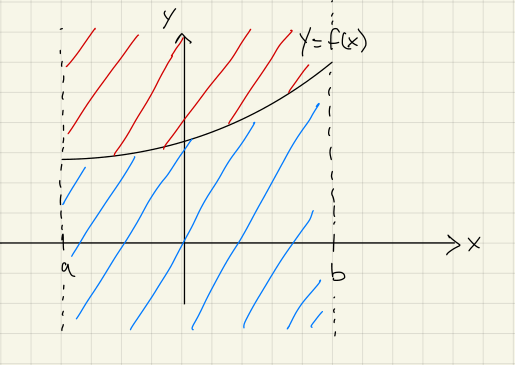
\includegraphics[width=0.45\textwidth]{grafico-di-funzioni-sopra-sotto.png}

\filbreak{}

\subsubsection*{Esempi}

\begin{enumerate}
    \item \(y \ge \ln(x)\) con \(0<x<2\)

          \medskip
          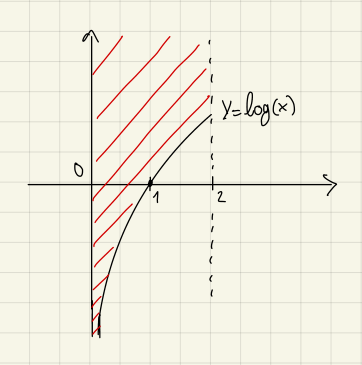
\includegraphics[width=0.4\textwidth]{grafico-di-funzioni-3.png}

    \item \(2x - 3y +1 \ge 0\)

          \(y \le \frac{2}{3}x + \frac{1}{3}\)

          \medskip
          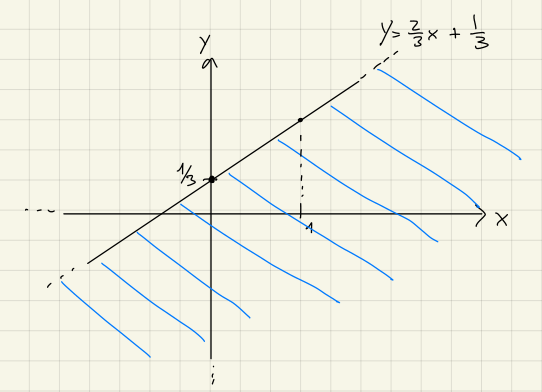
\includegraphics[width=0.5\textwidth]{grafico-di-funzioni-4.png}
\end{enumerate}

\filbreak{}
\subsubsection{Generalizzazione teorema degli zeri}

Vediamo come applicare il teorema degli zeri visto in \(\R \) per funzioni in \(\R^2\) attraverso un esempio.

Sia \(f(x,y) = x^2 - y^2 -1\) la nostra funzione. Vogliamo studiarne il segno e quindi vogliamo capire dove \(x^2-y^2 -1 \ge 0\). Iniziamo disegnando il grafico di quando \(f(x,y) = 0\), ovvero dell'iperbole:

\begin{center}
    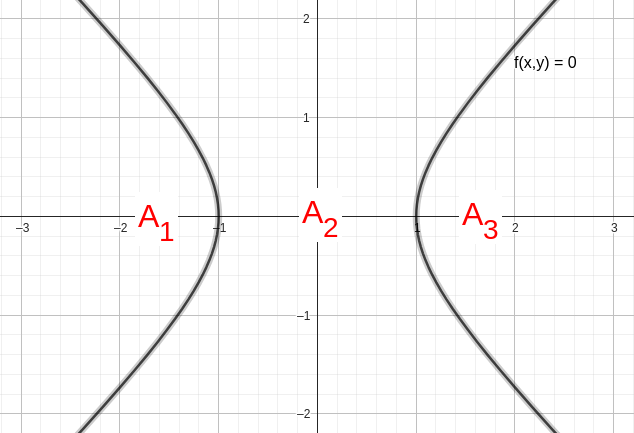
\includegraphics[width=0.5\textwidth]{teorema-degli-zeri-1.png}
\end{center}

Il grafico divide il piano nell zone \(A_1, A_2, A_3\) che sono insiemi aperti e connessi dove \(f(x,y) \ne 0\).

Con queste condizioni in ognuna delle zone il segno della funzione \underline{non} cambia.

(\textit{Generalizzazione teorema degli zeri})

Nel nostro caso \(f(x,y)\) è continua in \(\R^2\)

\(f(x,y)\) definisce un aperto del piano dato da un certo numero di aperti. Supponiamo che tali aperti siano in numero finito \(A_1, A_2, \ldots, A_n\)

Studio il segno di \(f(x,y)\) in ognuno di questi insiemi \(\underset{i=1, \ldots, n}{A_i}\).

In \(A_1\): \(f(x,y) \ne 0\) e dunque o \(f(x,y) > 0\) o \(f(x,y) < 0\). Essendo \(A_1\) aperto e connesso si ha che il segno di \(f(x,y)\), che è continua in \(A\), non cambia. Infatti, se esistessero due punti distinti di \(A_1\) in cui \(f(x,y)\) ha segno opposto, allora ci deve essere un punto in \(A_1\) in cui \(f(x,y) = 0\), ma \(f(x,y) \ne 0 ~\forall (x,y) \in A\).

In \(A_2, A_3\) si applica lo stesso ragionamento.

Studio quindi il segno in un punto comodo per ogni regione:

\begin{itemize}
    \item In \(A_1\): \(f(-2,0) = {(-2)}^2 + 0^2 - 1 = 3 > 0\)

          Dunque, \(f(x,y) > 0\) in \(A_1\) \((\forall (x,y) \in A_1)\)
    \item In \(A_2\): \(f(0,0) = 0^2 + 0^2 - 1 = -1 < 0\)

          Dunque, \(f(x,y) < 0\) in \(A_2\) \((\forall (x,y) \in A_2)\)
    \item In \(A_3\): \(f(2,0) = 2^2 + 0^2 - 1 = 3 > 0\)

          Dunque, \(f(x,y) > 0\) in \(A_3\) \((\forall (x,y) \in A_3)\)
\end{itemize}

Possiamo quindi aggiornare il grafico iniziale colorando le zone \(A_1\) e \(A_3\) dove \(f(x,y) > 0\).

\subsubsection*{Esempio}

Determinare l'insieme di definizione \(D \subset \R^2\) della seguente funzione, \(f: D \subseteq \R^2 \to \R \):

\[f(x,y) = \frac{\ln(x^3 - y)}{\sqrt{1-xy}}\]

Procediamo trovando il dominio della funzione:

\begin{align*}
    D & = \{(x,y) \in \R^2 \giventhat f(x,y) \in \R \}                      \\
      & = \{(x,y) \in \R^2 \giventhat (1-xy > 0) \text{ e } (x^3 -y > 0) \} \\
      & = \{(x,y) \in \R^2 \giventhat (xy < 1) \text{ e } (y < x^3) \}      \\
\end{align*}

Graficamente, è la parte di piano colorata in viola della seguente immagine:

\begin{center}
    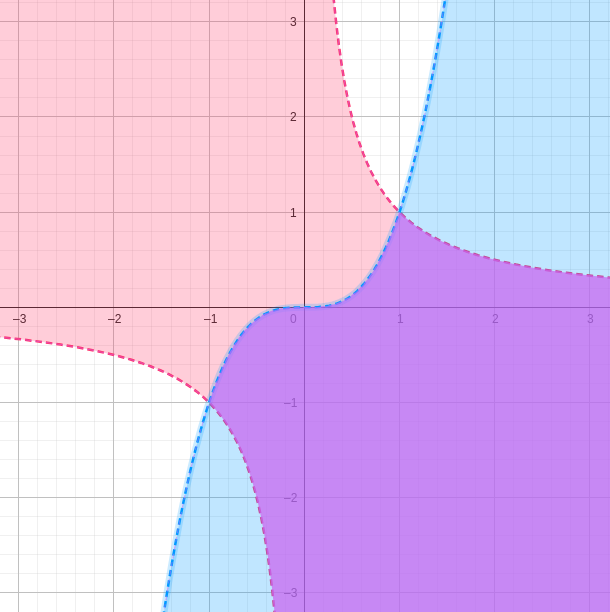
\includegraphics[width=0.6\textwidth]{esercizio-dominio-funzione-1.png}
\end{center}

\newpage
\subsubsection{Grafico di funzioni a due variabili}

Sia \(f: D \subseteq \R^2 \to \R \);

Il grafico di \(f(x,y)\) è un sottoinsieme \(S \subset \R^3 \).

\[\graf{f} = \{(x,y,z) \in \R^3 \giventhat z = f(x,y) \text{ con } (x,y) \in D\} \subset \R^3\]

\begin{center}
    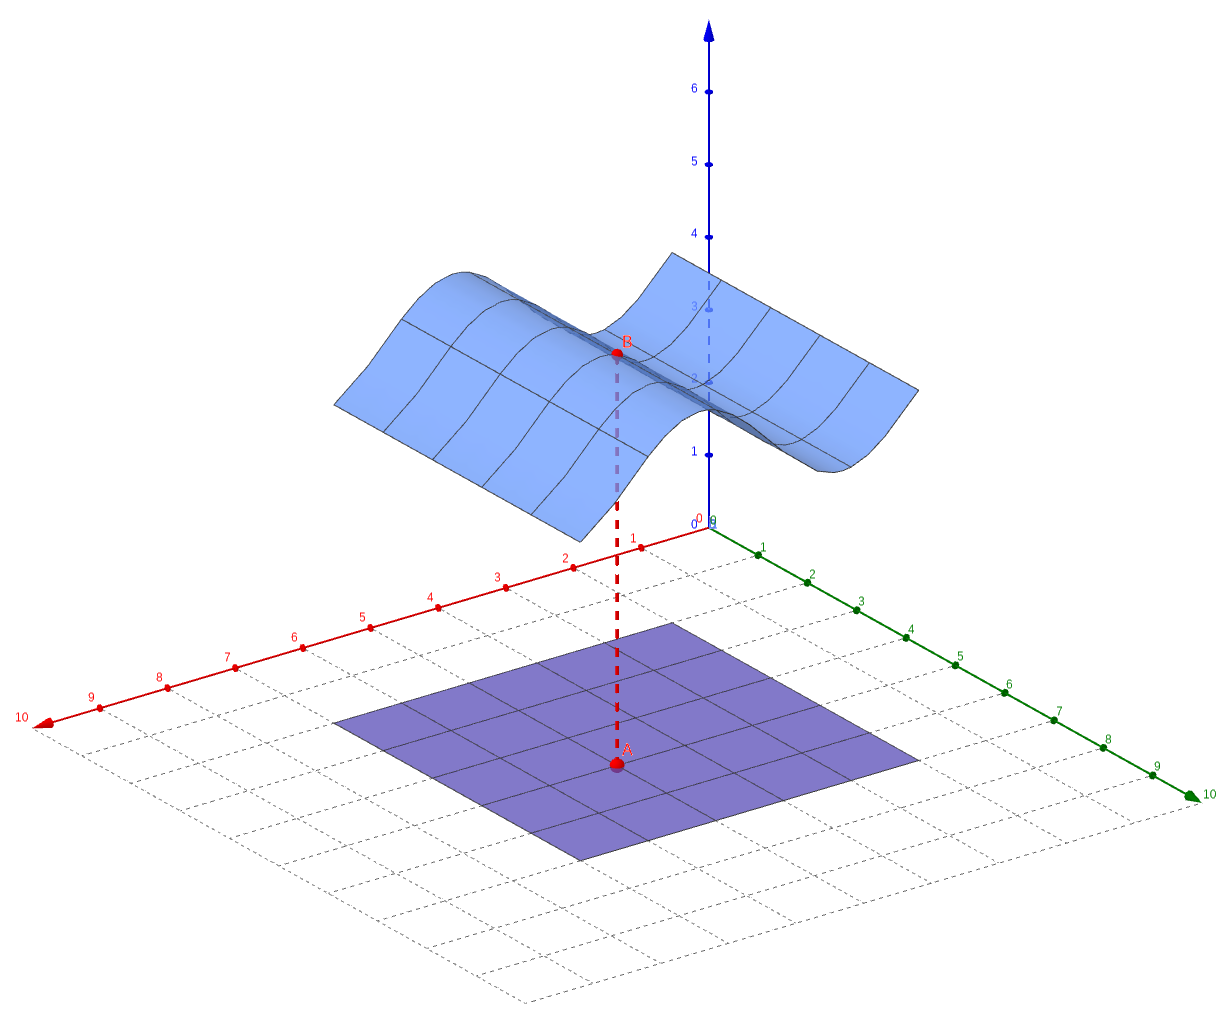
\includegraphics[width=0.8\textwidth]{grafico-di-funzione-2-variabili.png}
\end{center}

\begin{itemize}
    \item La nostra funzione \(f(x,y)\) è rappresentata con il colore celeste;
    \item La proiezione di \(S\) su \((x,y)\) è rappresentata con il colore viola;
    \item Dato un punto \((x,y,0) = A\), abbiamo il rispettivo punto \(B = (x,y,f(x,y))\)
    \item La distanza tra \(A\) e \(B\), rappresentata dal segmento tratteggiato, è chiamata ``Quota''.
\end{itemize}

Per studiare quindi il grafico di una funzione a 2 variabili, affetto il grafico con dei piani e studio le sezioni ottenute.

Le sezioni \underline{trasversali} intersecano \(S\) con i piani:
\begin{itemize}
    \item \(x=k\)
    \item \(y=k\)
    \item \(z=k \rightarrow \) piano orizzontale; otteniamo una sezione sul piano \((x,y)\)
\end{itemize}

Queste sono chiamate \textbf{Tracce} della funzione e si definiscono come segue:

\[
    S \subset \R^3\
    \begin{cases}
        \graf{f} \\
        x=k
    \end{cases}
    \implies
    \begin{cases}
        z = f(x,y) \\
        x=k
    \end{cases}
    \implies
    z = f(k,y) \quad \text{grafico nel piano }(y,z)
\]
\[
    S \subset \R^3\
    \begin{cases}
        \graf{f} \\
        y=k
    \end{cases}
    \implies
    \begin{cases}
        z = f(x,y) \\
        y=k
    \end{cases}
    \implies
    z = f(x,k) \quad \text{grafico nel piano }(x,z)
\]
\[
    S \subset \R^3\
    \begin{cases}
        \graf{f} \\
        z=k
    \end{cases}
    \implies
    \begin{cases}
        z = f(x,y) \\
        z=k
    \end{cases}
    \implies
    k = f(k,y) \quad \text{grafico nel piano }(x,y)
\]

Le intersezioni del grafico con i piani \(z=k\) sono chiamate \textbf{insiemi di livello K} della funzione.

Queste sono anche chiamate \textbf{curve di livello} se relative a ``curve'', ovvero se la funzione non è costante. Queste sono curve lungo le quali la funzione \(f(x,y)\) assume lo stesso valore \(f(x,y) = k\).

\subsubsection{Insiemi o curve di livello}

Come abbiamo appena visto, le \textbf{curve di livello} sono le intersezioni del grafico con il piano \(z=k\).

Vediamo la questione in pratica; prendiamo la funzione, \(f: \R^2 \to \R \), definita da:
\[
    f(x,y) = x^2 + y^2
\]
L'insieme delle curve di livello si scrive:

\[
    E_k = \left\{ (x,y) \in \R^{2} \giventhat x^{2}+y^{2}=k \right\}
\]

Se consideriamo i punti \((x,y)\) che stanno nell'insieme di livello \(k=1\) della funzione, questi sono i punti che stanno sulla circonferenza di centro \((0,0)\) di raggio 1:

\[
    E_1 = \left\{ (x,y) \in \R^{2} \giventhat x^{2}+y^{2}=1 \right\}
\]

\begin{center}
    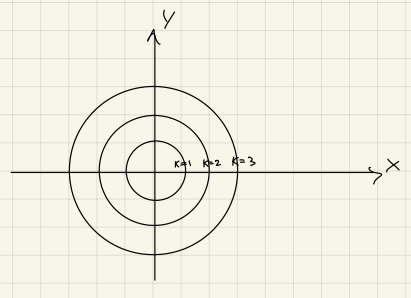
\includegraphics[width=0.5\textwidth]{curve-di-livello-esempio.png}
\end{center}

\filbreak{}
Quindi il grafico di \(f\) ha la seguente forma:

\begin{center}
    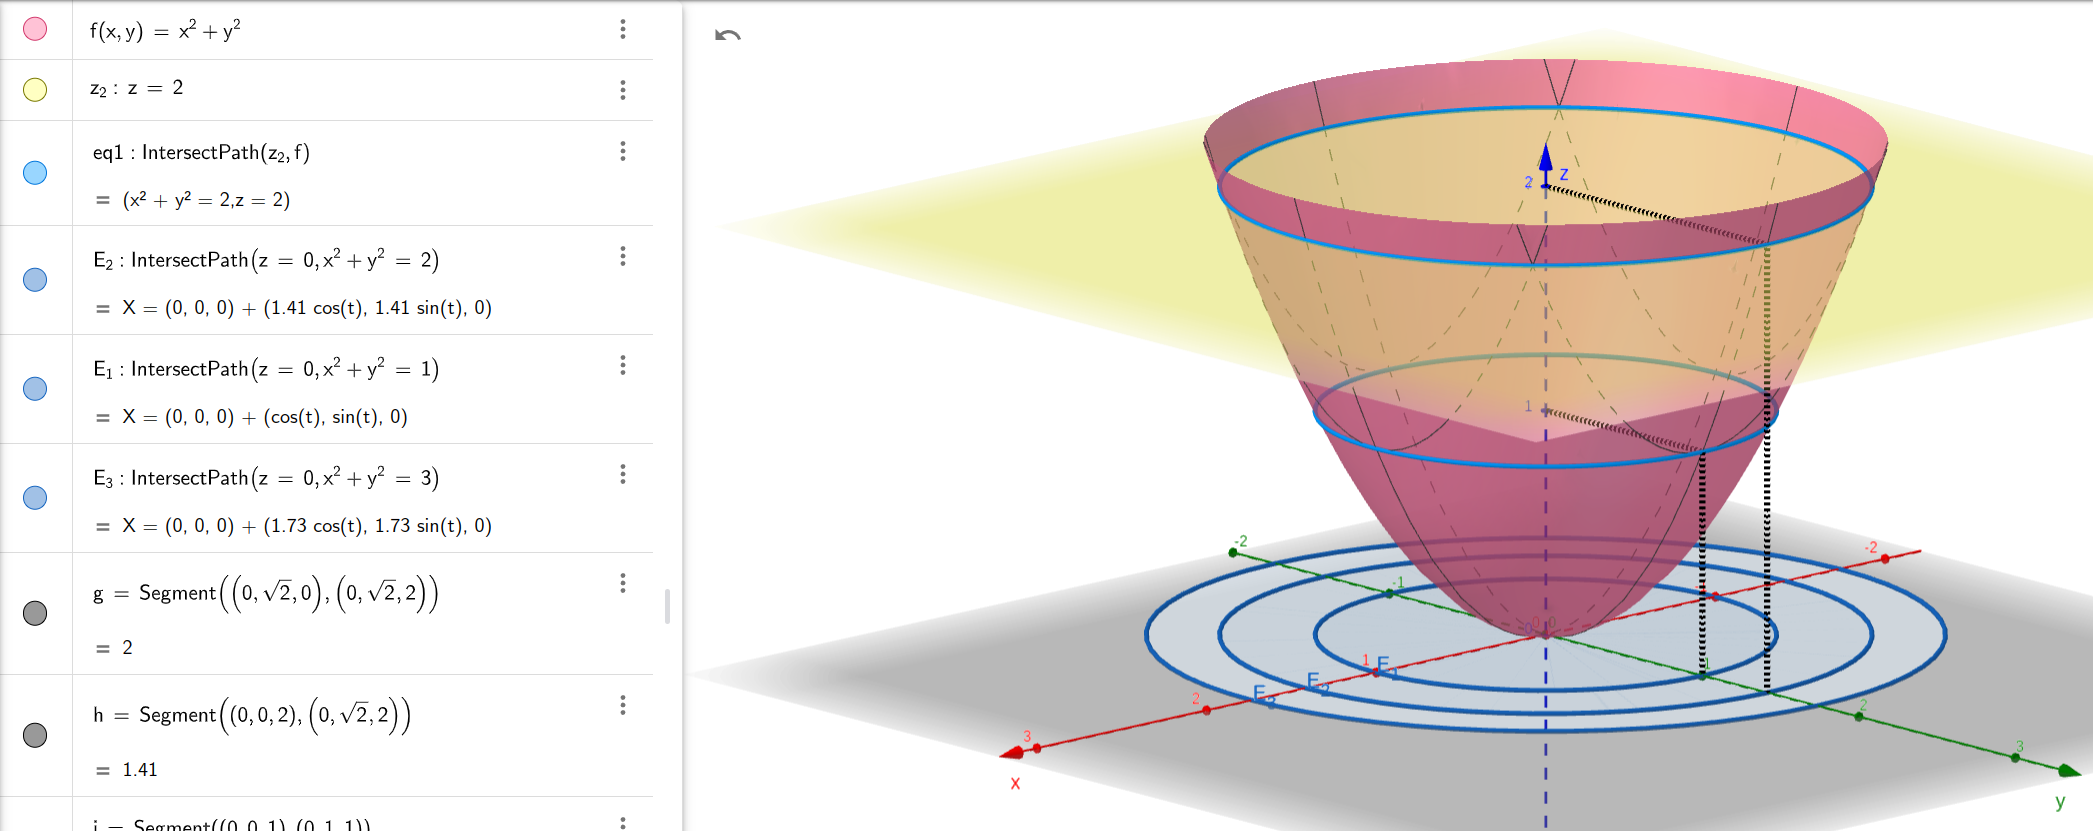
\includegraphics[width=\textwidth]{curve-di-livello-esempio-2.png}
\end{center}

\pagebreak
\subsubsection{Esempi {-} Domini}

\subsubsection*{Esempio 1}

Determinare l'insieme di definizione della seguente funzione:

\[
    z = \sqrt{1-x^{2}-y^{2}}
\]

\(D = \{(x,y) \in \R^2 \giventhat f(x,y) \in \R \} = \{(x,y) \in \R^{2} \giventhat x^{2}+y^{2} \le 1\} \)

Questo vuol dire che la funzione è definita all'interno della circonferenza di funzione:
\[
    f(x,y) = x^2+y^2-1
\]

Essendo questa una circonferenza di raggio 1 con centro l'origine degli assi, possiamo dire che il dominio \(D\) costituito dai punti interni a questa circonferenza è chiuso.

Inoltre, possiamo analizzare le curve di livello:
\[
    E_k = \{(x,y) \in D \giventhat x^2+y^2=1+k\}
\]
Quindi:
\begin{itemize}
    \item \(k<-1 \implies E_k = \emptyset \)
    \item \(-1\le k \le 0 \implies E_k = \{(x,y)\in \R^{2} \giventhat x^2+y^2=1+k\} \)
    \item \(k>0 \implies E_k = \emptyset \)
\end{itemize}

\filbreak{}
\subsubsection*{Esempio 2}

Determinare l'insieme di definizione della seguente funzione:

\[
    z = \sqrt{1-x^{2}}+\sqrt{1-y^{2}}
\]

devo imporre il dominio:

\[
    \{(x,y) \in \R^{2} \giventhat x^{2}\le 1;\ y^{2}\le 1\}
\]

Quindi abbiamo quattro piani che si intersecano, due per \(x^2=1\) e due per \(y^2=1\).

\begin{center}
    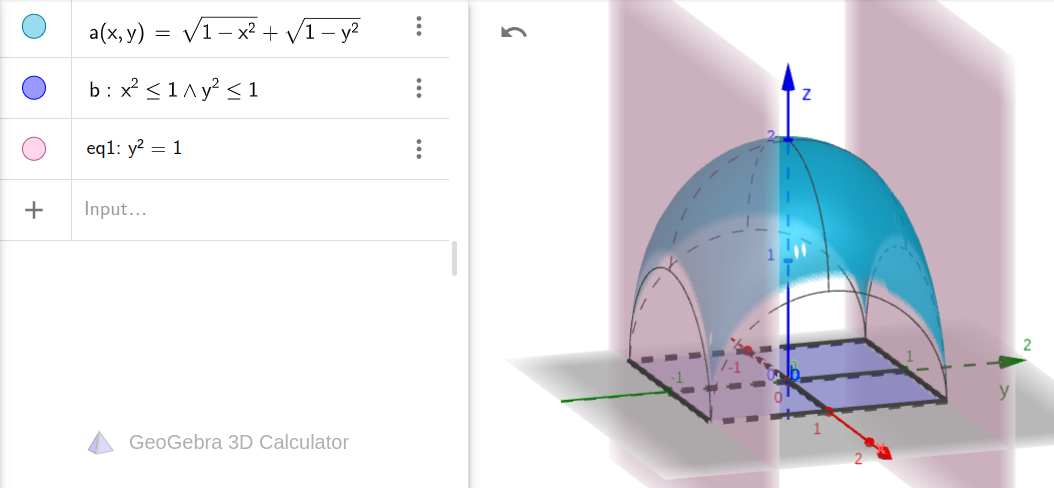
\includegraphics[width=\textwidth]{curva-di-livello-2.png}
\end{center}

Quindi il dominio \(D\) è chiuso.

\pagebreak
\subsubsection*{Esempio 3}

Determinare l'insieme di definizione della seguente funzione:

\[
    z = \frac{1}{\sqrt{y-\sqrt{x}}}
\]

\[
    D=\{(x,y) \in \R^{2} \giventhat y-\sqrt{x}>0,\ x \ge 0\}
\]

Vuole dire che prendiamo solo i valori che stanno a destra dell'asse y e nel sopragrafico della seguente parabola.

\begin{center}
    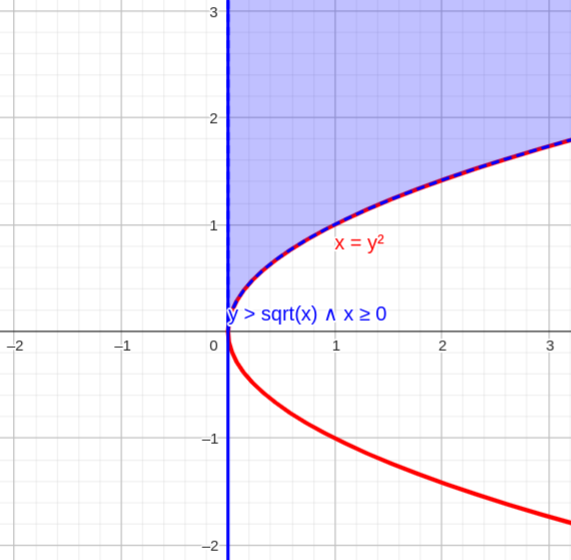
\includegraphics[width=0.65\textwidth]{curva-di-livello-3.png}
\end{center}

\pagebreak
\subsubsection{Esercizi {-} Insiemi di livello}

\subsubsection*{Esercizio 1}

Determinare gli insiemi di livello della seguente funzione:

\[
    z = x+2y
\]

Il dominio è tutto \(\R^2\).

\[
    E_k = \{(x,y) \in \R^2 \giventhat x+2y = k\} = \left\{(x,y) \in \R^2 \giventhat[\bigg] y = \frac{k-x}{2}\right\} \to \text{fascio di rette}
\]

\filbreak{}
\subsubsection*{Esercizio 2}

Determinare gli insiemi di livello della seguente funzione:

\[
    z = x^{2}+9y^{2}
\]

Il dominio è tutto \(\R^2\).

\[
    E_k = \{(x,y) \in \R^{2}\ \vert\ x^{2}+9y^{2}=k\}
\]

se \(k<0\): \(E_k = \emptyset \)

se \(k=0\): \(E_0=(0,0)\) ovvero l'origine degli assi

se \(k>0\): otteniamo delle ellissi:

\[
    \frac{x^{2}}{9}+ y^{2} = \frac{k}{9}
\]

\filbreak{}
\subsubsection*{Esercizio 3}

Determinare gli insiemi di livello della seguente funzione:

\[
    z= \frac{y}{x^{2}}
\]

dominio

\[
    E_k = \{(x,y) \in \R^{2} \giventhat x+2y=k\}
\]

\[
    y=-\frac{1}{2} + \frac{x}{2}
\]

Fascio di rette parallele a \(y = -\frac{1}{2}x\)

\filbreak{}
\subsubsection*{Esercizio 4}

Determinare gli insiemi di livello della seguente funzione:

\[
    z= \frac{y}{x^{2}}
\]

dominio:

\[
    E_k = \left\{(x,y) \in \R^{2} \giventhat[\Big] x \neq  0;\ \frac{y}{x^{2}}=k \right\}
\]

se \(k=0\), è \(E_0\) privata dell'origine:

\[
    \frac{y}{x^{2}}=0
\]

se \(k \ne 0\):

\[
    \frac{y}{x^{2}} = k
\]

\[
    y = kx^{2}
\]

\vspace{5mm}
\begin{center}
    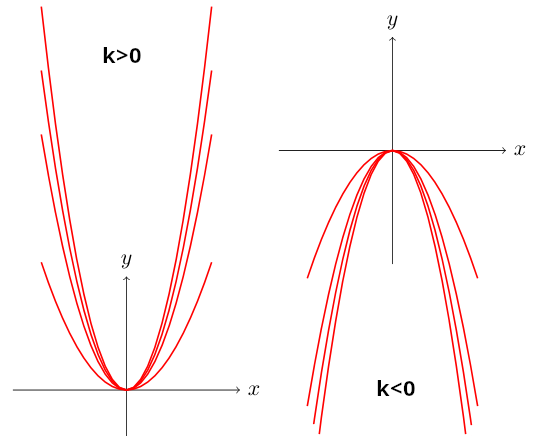
\includegraphics[width=0.6\textwidth]{insiemi-di-livello-esempio-4.png}
\end{center}

\filbreak{}
\subsubsection*{Esercizio 5}

Studiare gli insiemi di livello della seguente funzione:

\[
    z = \frac{2x}{x^2+y^2}
\]

Notiamo le condizioni di esistenza del denominatore:

\[f(x,y) = x^2 + y^2 \to f: \R^2 \setminus \{\uzero \} \to \R \]

Per cui gli insiemi di livello sono:

\[E_k = \left\{ (x,y) \in \R^2 \setminus \{(0,0)\} \giventhat[\bigg] \frac{2x}{x^2+y^2} = k \right\} \]

Se \(k=0\):

\[
    \frac{2x}{x^2+y^2} = 0 \implies x = 0;\ y \ne 0 \qquad \text{ovvero tutti i punti sull'asse \(y\) eccetto l'origine.}
\]

Se \(k \ne 0\):
\begin{align*}
    \frac{2x}{x^2+y^2} = k & \implies 2x = k (x^2+y^2) \implies kx^2 + ky^2 -2x = 0                                                        \\
                           & \implies x^2 + y^2 -\frac{2}{k}x = 0 \implies {\left( x-\frac{1}{k} \right)}^2 + y^2 = \frac{1}{k^2}          \\
                           & \text{ovvero le circonferenze di centro } c=\left( \frac{1}{k}, 0 \right) \text{ e raggio } r = \frac{1}{|k|}
\end{align*}
\begin{center}
    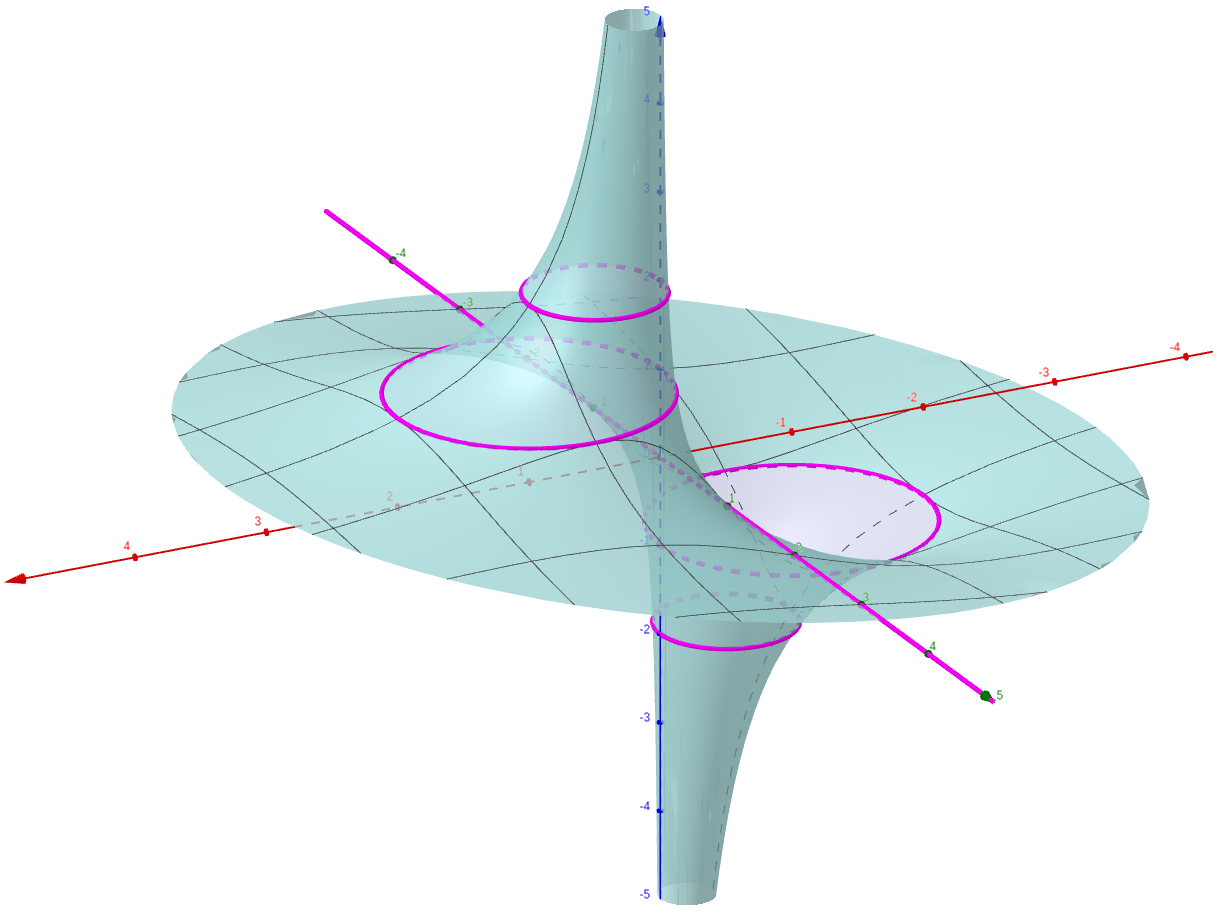
\includegraphics[width=0.7\textwidth]{insiemi-di-livello-esempio-5.png}
\end{center}

\pagebreak
\subsubsection{Esercizi {-} limiti}

\subsubsection*{Esercizio 1}

\[
    \lim_{ (x,y) \to (0,0) } \frac{xy(2y^{2}+x^{3})}{x^{4}+y^{2}}
\]

Sostituendo \((x,y)\) con \((0,0)\) otteniamo una forma indeterminata.

Consideriamo dunque le restrizione della funzione lungo le rette \(y=mx\):

\[
    \lim_{\begin{smallmatrix}(x,y) \to (0,0) \\ y=mx\end{smallmatrix}} f(x,y) = \lim_{\begin{smallmatrix}(x,y) \to (0,0) \\ y=mx\end{smallmatrix}} \frac{xmx(2m^{2}x^{2}+x^{3})}{x^{4}+m^{2}x^{2}}= \lim_{ x \to 0 } \frac{mx^{2}(2m^{2}+x)}{(x^{2}+m^{2})} = 0
\]

il limite quindi se esiste deve essere zero. Passiamo adesso alle coordinate polari per valutare \(f\):

\begin{spreadlines}{3mm}
    \begin{align*}
        \left|f(\rho, \theta)\right| & = \left|\frac{\rho\cos(\theta) \rho\sin(\theta) (2\rho^{2}\sin^{2}(\theta)+\rho^{3}\cos^{3}(\theta))}{\rho^{4}\cos^{4}(\theta)+\rho^{2}\sin^{2}(\theta)}\right| \\
                                     & = \left|\frac{\rho^{2}\cos(\theta) \sin(\theta) (2\sin^{2}(\theta)+\rho \cos^{2}(\theta))}{\rho^{2}\cos^{4}(\theta)+\sin^{2}(\theta)} \right|                   \\
                                     & \le \left|\rho^{2}\cos(\theta) \sin(\theta) (2\sin^{2}(\theta)+\rho \cos^{2}(\theta))\right|                                                                    \\
                                     & = \left|2\rho^{2}\cos(\theta)\sin^3(\theta) + \rho^{3}\cos^3(\theta)\sin(\theta)\right|                                                                         \\
                                     & \le 2\rho^2|\cos(\theta)\sin^3(\theta)| + \rho^2|\rho\cos^3(\theta)\sin(\theta)|                                                                                \\
                                     & \le 2\rho^2 + \rho^4 \xrightarrow[\rho \to 0^+]{} 0
    \end{align*}
\end{spreadlines}

Il limite di \(f(x,y)\) per \((x,y) \to (0,0)\) dunque esiste e vale \(0\).

Per dimostrarlo, potevamo usare anche un altro metodo senza passare alle coordinate polari:

\[
    \left|f(x,y)\right| =  \left|\frac{xy(2y^{2}+x^{3})}{x^{4}+y^{2}}\right| = \left|\frac{2xy^{3}+x^{4}y}{x^{4}+y^{2}}\right| = \left| \frac{2xy^{3}}{x^{4}+y^{2}}+ \frac{x^{4}y}{x^{4}+y^{2}}\right| \le \left|\frac{2xy^{3}}{x^{4}+y^{2}}\right|+ \left|\frac{x^{4}y}{x^{4}+y^{2}}\right|
\]

quindi:

\[
    |f(x,y)|  \le \frac{2|xy^{3}|}{x^{4}+y^{2}} + \frac{x^{4}|y|}{x^{4}+y^{2}} \le \frac{2|xy^{3}|}{y^{2}} + \frac{x^{4}|y|}{x^{4}}
\]

\[
    |f(x,y)|  \le \underbrace{2 |xy| + |y|}_{g(x,y)}
\]

La funzione \(g\) è continua su tutto \(\R \) ed è inoltre \(\ge 0\). Dunque, il limite è:

\[
    \lim_{ (x,y) \to (0,0) } g(x,y) = g(0,0) = 0
\]

Quindi per il teorema del confronto, 0 è effettivamente il limite di \(f(x,y)\) per \((x,y) \to (0,0)\)

\filbreak{}
\subsubsection*{Esercizio 2}

\[
    \lim_{ (x,y) \to (0,0) } \frac{x\sin^{2}(y)+ 3xy^{4}}{x^{2}+2y^{4}}
\]

Sostituendo \((x,y)\) con \((0,0)\) otteniamo una forma indeterminata.

riscrivo la \(f\) come somma di due funzioni:

\[
    f(x,y) = \frac{x\sin^{2}(y)+ 3xy^{4}}{x^{2}+2y^{4}}  = \underbrace{\frac{x\sin^{2}(y)}{x^{2}+2y^{4}}}_{f_1(x,y)} + \underbrace{\frac{3xy^{4}}{x^{2}+2y^{4}}}_{f_2(x,y)}
\]

Affinché \(f(x,y)\) abbia limite, anche \(f_1, f_2\) devono averlo.

Vediamo prima \(f_2\) che è più semplice.

\[
    |f_2(x,y)| = \left| \frac{3xy^{4}}{x^{2}+2y^{4}}\right| =\frac{3y^{4}|x|}{x^{2}+2y^{4}} \le \frac{3y^{4}|x|}{2y^{4}} = \frac{3}{2}|x| \rightarrow 0
\]

Dunque, \(f_2(x,y) \xrightarrow[(x,y) \to (0,0)]{} 0\).

Vediamo ora \(f_1\):

\[
    f_1(x,y) = \frac{x\sin^{2}y}{x^{2}+2y^{4}}
\]

Notiamo che se passiamo alle coordinate polari, il numeratore va come \(\rho^{3}\), mentre il denominatore come \(\rho^{4}\). Il limite potrebbe quindi non esistere, controlliamolo.

Ricordando che \(\sin(x) \xrightarrow[x \to 0]{} 0\);

Guardo la funzione lungo il cammino \(y=x\):

\[
    \lim_{ \begin{smallmatrix}(x,y) \to (0,0) \\ y=x \end{smallmatrix} } f_1(x,y) = \lim_{ x \to 0 } \frac{x\sin^{2}(x)}{x^{2}+2x^{4}} = \lim_{ x \to 0 } \frac{x\sin^{2}(x)}{x^{2}(1+2x^{2})} = \lim_{ x \to 0 } \frac{x}{1+2x^2} = 0
\]

Per \(x = y^{2}\):

\[
    \lim_{ \begin{smallmatrix}(x,y) \to (0,0) \\ x=y^2 \end{smallmatrix} } f_1(x,y)  = \lim_{ y \to 0 } \frac{y^{2}\sin^{2}(y)}{y^{4}+2y^{4}} = \lim_{ y \to 0 } \frac{\sin^{2}(y)}{3y^{2}}  = \frac{1}{3}
\]

quindi il limite non esiste perché \(f= f_1+f_2\) ma \(\lim_{ (x,y) \to (0,0) } f_1\) non esiste.

\pagebreak
\subsubsection{Scelta delle curve di restrizione}

Nell'esercizio di prima come ho fatto a restringere la \(f_1\)?

Vediamolo:

\begin{itemize}
    \item \(y=x\), peso le variabili allo stesso modo e dunque dal denominatore (\(x^{2}+2y^{4}\)) ottengo \(x^{2}+2x^{4}\). Quindi, per \(x \rightarrow 0\), sto dando più importanza al monomio \(x^2\).
    \item \(x=y^{2}\), dal denominatore (\(x^{2}+2y^{4}\)) ottengo \(y^{4}+2y^{4} = 3y^{4}\) quindi qua non trascuro gli addendi che ora hanno lo stesso peso.
\end{itemize}

In generale, quindi, quando si cerca di verificare la \textbf{NON ESISTENZA} del limite, si prova a vedere cosa fa la funzione dando pesi diversi alle vari parti che la compongono.

\subsubsection*{Esempio}

\[
    \lim_{ (x,y) \to (0,0) } \left( \left( \frac{xy^{2}+2y^{ \frac{1}{3}}\sin^{2}(x)}{x^{2}+y^{2}}\right) \cdot e^{ \left(\frac{x^{2}-y^{2}}{x^{2}+y^{2}}\right)} \right)
\]

L'esponente dell'esponenziale, preso da solo, abbiamo già verificato che non ha limite. Se però riusciamo a dimostrare che esiste il limite per la prima parentesi, e inoltre riusciamo a limitare uniformemente l'esponenziale, allora abbiamo un limite per il tutto.

Vediamo l'esponente dell'esponenziale:

\[
    \frac{x^{2}-y^{2}}{x^{2}+y^{2}} \le \left|\frac{x^{2}-y^{2}}{x^{2}+y^{2}}\right| = \frac{\left|x^{2}-y^{2}\right|}{x^{2}+y^{2}}  \le \frac{\left|x^{2}\right|+\left|y^{2}\right|}{x^{2}+y^{2}} = \frac{x^{2}+y^{2}}{x^{2}+y^{2}} = 1
\]
quindi:
\[
    0 < e ^{ \frac{x^{2}-y^{2}}{x^{2}+y^{2}}} \le e
\]

Buono, a noi non da noia che sta tra \(0\) ed \(e\), ci importa solo che il limite esiste e non tende all'infinito.

Studiamo ora l'altra parte della funzione \(f(x,y)\) usando le coordinate polari:

\begin{align*}
    \left| \frac{\rho\cos(\theta) \rho^{2}\sin^{2}(\theta) + 2 \rho^{\frac{1}{3}}\sin^{\frac{1}{3}}(\theta) \sin^{2}(\rho\cos(\theta))}{\rho^{2}}\right| & \le \left| \frac{\rho^{3}\cos(\theta)\sin^{2}(\theta)}{\rho^{2}}\right| + \left|\frac{2 \rho^{\frac{1}{3}}\sin^{\frac{1}{3}}(\theta) \sin^{2}(\rho\cos(\theta)) }{\rho^{2}}\right| \\
                                                                                                                                                         & \le \left| \rho\cos(\theta) \sin ^{2}(\theta)\right| + \left|\frac{2 \rho^{\frac{1}{3}} \sin^{\frac{1}{3}}(\theta) \rho^2\sin^{2}(\cos(\theta)) }{\rho^{2}}\right|                 \\
                                                                                                                                                         & \le \left| \rho\cos(\theta) \sin ^{2}(\theta)\right| + \left| 2 \rho^{\frac{1}{3}} \sin^{\frac{1}{3}}(\theta) \sin^{2}(\cos(\theta)) \right|                                       \\
                                                                                                                                                         & \le \left| \rho\cos(\theta) \sin ^{2}(\theta)\right| + 2 \rho^{ \frac{1}{3}} \left| \sin^{\frac{1}{3}}(\theta) \cos^{2}(\theta)\right|                                             \\
                                                                                                                                                         & \le \rho + 2 \rho^{ \frac{1}{3}} \xrightarrow[\rho \to 0^+]{} 0
\end{align*}

quindi alla fine il limite è:

\[
    \lim_{ (x,y) \to (0,0) } f(x,y) = 0 \cdot e = 0
\]
